\chapter{Appendix}
    \begin{figure}[h]
        \centering
        % 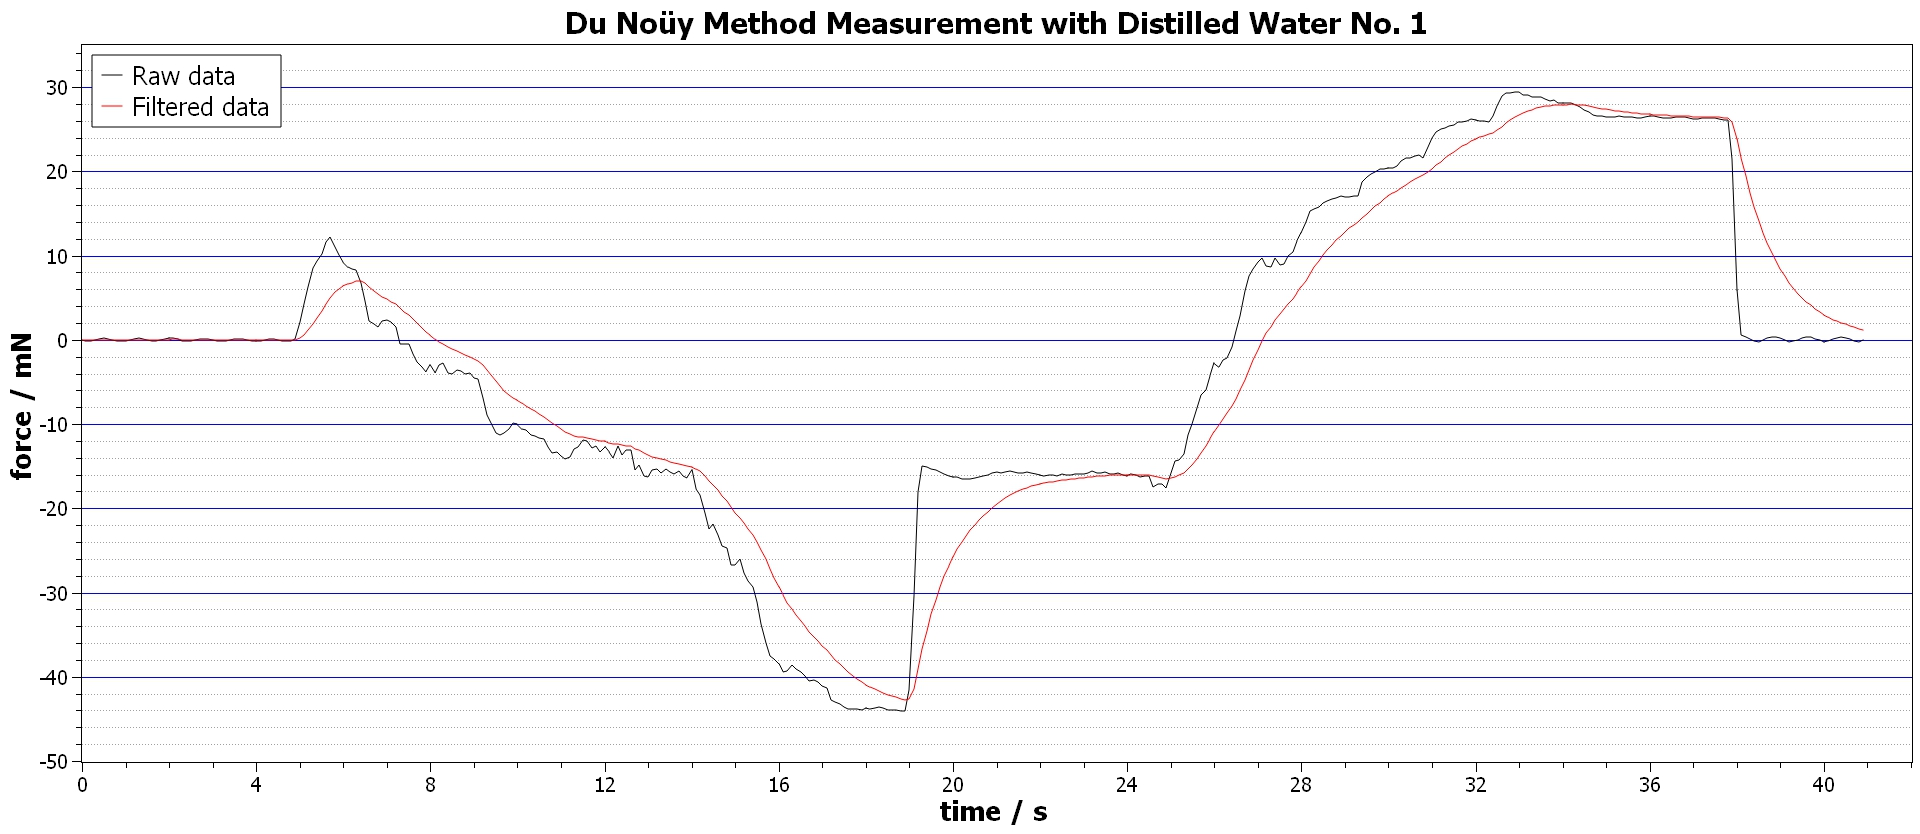
\includegraphics[width=.9\textwidth]{scidavis/Du_Nouy_Method_Measurement_with_distilled_water_No_1.jpg}
        \includesvg[inkscapelatex=false, width=.9\textwidth]{scidavis/Du_Nouy_Method_Measurement_with_distilled_water_No_1}
        \caption[Measurement with \textsc{Du Noüy} ring in distilled water (\(\vartheta \approx \SI{20}{\celsius}\))]{Measurement with \textsc{Du Noüy} ring in distilled water (\(\vartheta \approx \SI{20}{\celsius}\)).}
        \label{fig:Du_Nouy_Method_Measurement_with_distilled_water_No_1}
    \end{figure}
    \begin{figure}[h]
        \centering
        % 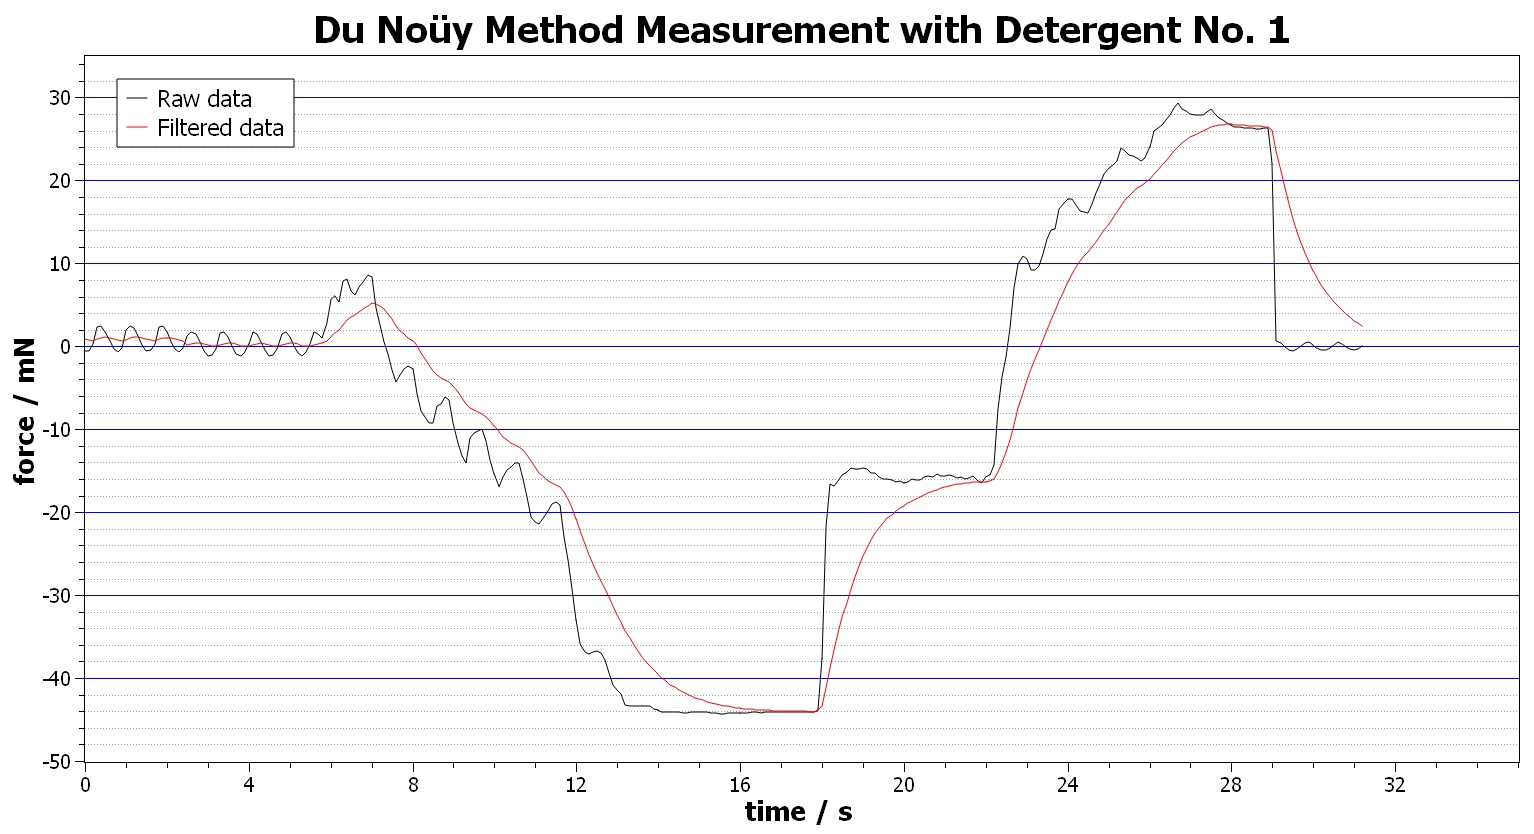
\includegraphics[width=.9\textwidth]{scidavis/Du_Nouy_Method_Measurement_with_detergent_No_1.jpg}
        \includesvg[inkscapelatex=false, width=.9\textwidth]{scidavis/Du_Nouy_Method_Measurement_with_detergent_No_1}
        \caption[Measurement with \textsc{Du Noüy} ring in detergent (\(\vartheta \approx \SI{20}{\celsius}\))]{Measurement with \textsc{Du Noüy} ring in detergent (\(\vartheta \approx \SI{20}{\celsius}\)).}
        \label{fig:Du_Nouy_Method_Measurement_with_detergent_No_1}
    \end{figure}
    \begin{figure}[h]
        \centering
        % 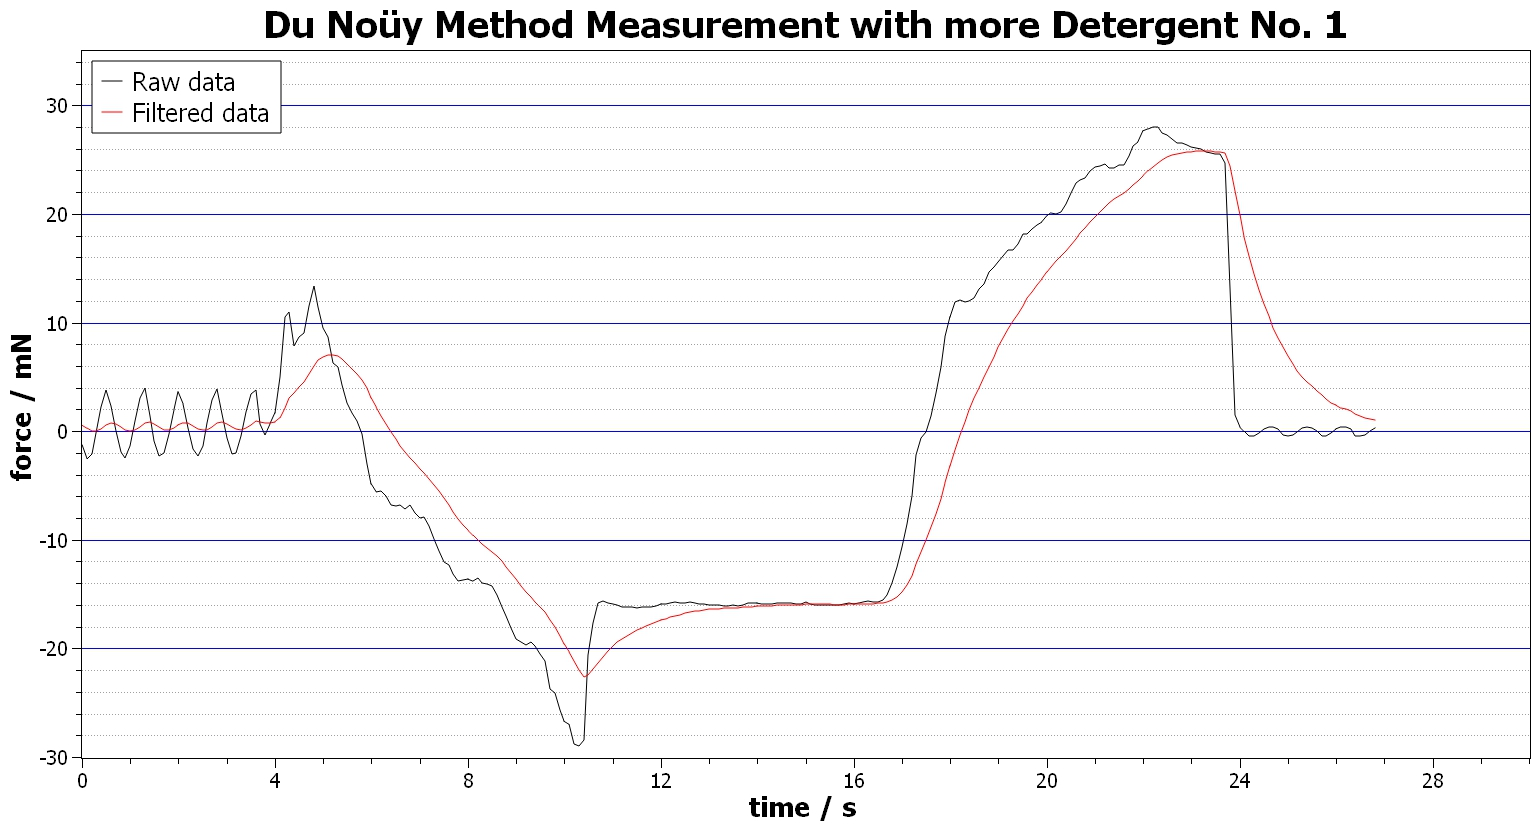
\includegraphics[width=.9\textwidth]{scidavis/Du_Nouy_Method_Measurement_with_more_detergent_No_1.jpg}
        \includesvg[inkscapelatex=false, width=.9\textwidth]{scidavis/Du_Nouy_Method_Measurement_with_more_detergent_No_1}
        \caption[Measurement with \textsc{Du Noüy} ring in a larger amount of detergent (\(\vartheta \approx \SI{20}{\celsius}\))]{Measurement with \textsc{Du Noüy} ring in a larger amount of detergent (\(\vartheta \approx \SI{20}{\celsius}\)).}
        \label{fig:Du_Nouy_Method_Measurement_with_more_detergent_No_1}
    \end{figure}
    \begin{figure}[h]
        \centering
        % 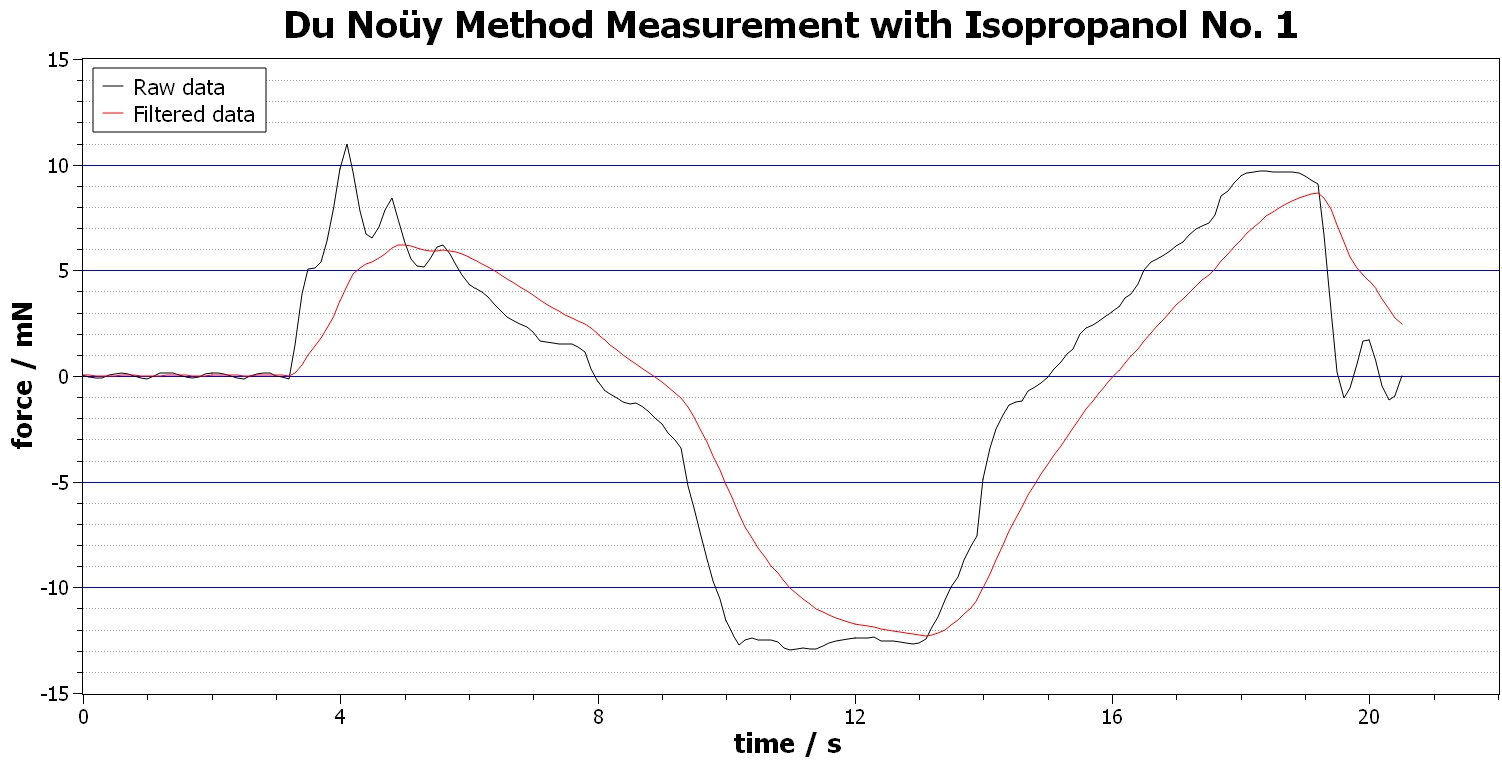
\includegraphics[width=.9\textwidth]{scidavis/Du_Nouy_Method_Measurement_with_isopropanol_No_1.jpg}
        \includesvg[inkscapelatex=false, width=.9\textwidth]{scidavis/Du_Nouy_Method_Measurement_with_isopropanol_No_1}
        \caption[Measurement with \textsc{Du Noüy} ring in isopropanol (\(\vartheta \approx \SI{20}{\celsius}\))]{Measurement with \textsc{Du Noüy} ring in isopropanol (\(\vartheta \approx \SI{20}{\celsius}\)).}
        \label{fig:Du_Nouy_Method_Measurement_with_isopropanol_No_1}
    \end{figure}
    % \newpage
\chapter{Appendix}
    \begin{figure}[h]
        \centering
        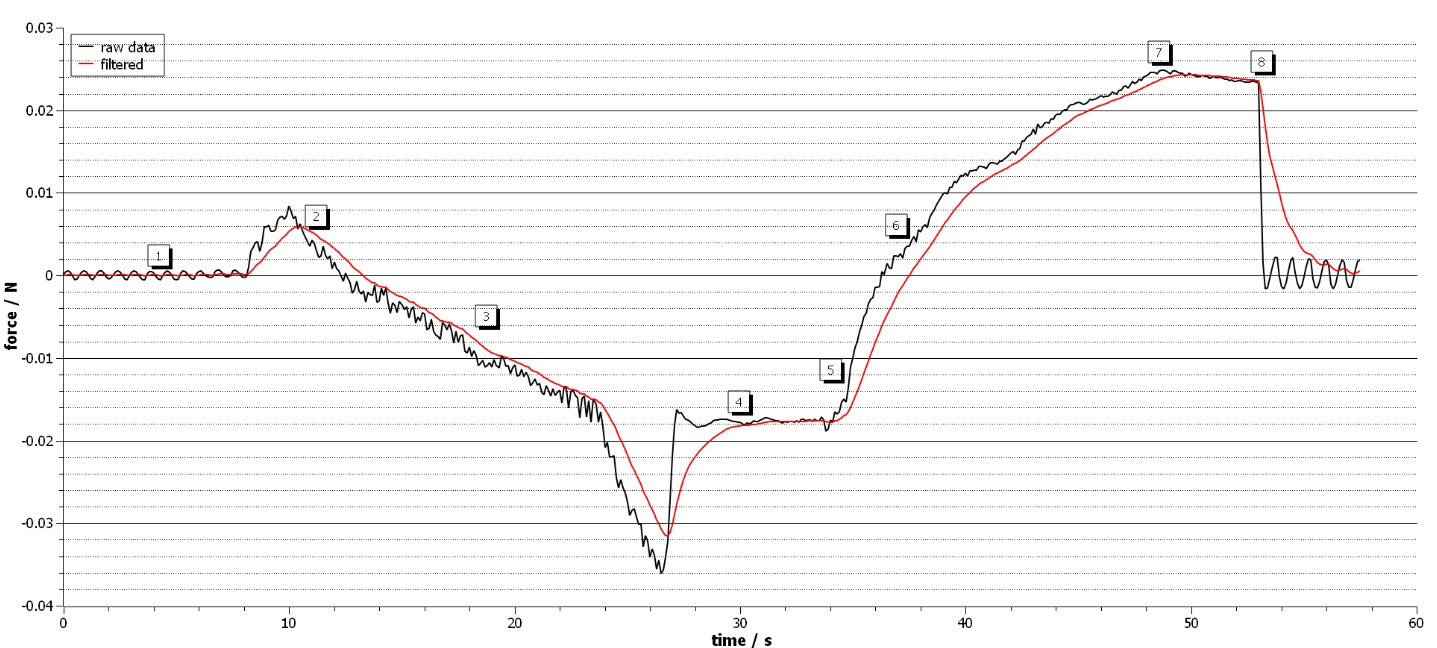
\includegraphics[width=.9\textwidth]{referenzen/instructions_fig14.jpg}
        \caption[Expected profile of the force-time diagram]{Expected profile of the force-time diagram with enumerated marks on significant regions.}
        \label{fig:instructions_fig14}
    \end{figure}
\newpage
\chapter{Appendix}
%
% \inputencoding{ascii}
\lstinputlisting[caption={\textsc{MATLAB} script to simulate the step response of an exponential filter algorithm.}, label={code:step response}, style=MatLAB]{MatLAB/step_response/step_response.m}
\newpage
\lstinputlisting[caption={\textsc{MATLAB} script to apply an exponential filter to the GISTEMP v4 data set provided by the Goddard Institute of
    Space Studies \cite{GISS.nasa.surface.temperature.analysis.20210120}.}, label={code:expo filter matlab}, style=matlab]{matlab/noisy_data/exposmooth_noise.m}
\newpage
\lstinputlisting[caption={\textsc{MATLAB} script to import the data set.}, label={code:import GISTEMP dataset matlab}, style=matlab]{matlab/noisy_data/generated_table_import.m}
